\documentclass[10pt]{beamer}
\usepackage{amsmath}
\usepackage{amssymb}
\usepackage{geometry}
\usepackage{graphicx}
\usepackage{url}

% some latex magic for correcting apostrophe issue in verbatim mode
\makeatletter
\let \@sverbatim \@verbatim
\def \@verbatim {\@sverbatim \verbatimplus}
{\catcode`'=13 \gdef \verbatimplus{\catcode`'=13 \chardef '=13 }} 
\makeatother

\begin{document}

%-------------------------------------------
\begin{frame}
\large
Lecture 1\\
Simple Linear Regression\\
STAT 632, Spring 2020
\end{frame}

%-------------------------------------------
\begin{frame}{Introduction}
\begin{itemize}
\item Regression analysis is a method for investigating the functional relationship among variables.  It is a useful method for predicting values of one variable using one or more other variables. 
\vspace{10pt}
\item \textbf{Simple linear regression} (SLR) involves modeling the relationship between two variables as a straight line, i.e., $Y$ is modeled as a linear function of $X$.
\end{itemize}
\end{frame}

%-------------------------------------------
\begin{frame}[fragile]{Example}
A scatterplot of weight ($Y$) versus height ($X$) for 247 physically active men.
\small
\begin{verbatim}
> library(openintro)
> bdims_males <- subset(bdims, sex == 1) 
> plot(wgt ~ hgt, data = bdims_males, 
    xlab = 'Height (cm)', ylab = 'Weight (kg)', cex=0.5)
\end{verbatim}
\begin{figure}[htbp]
\centering
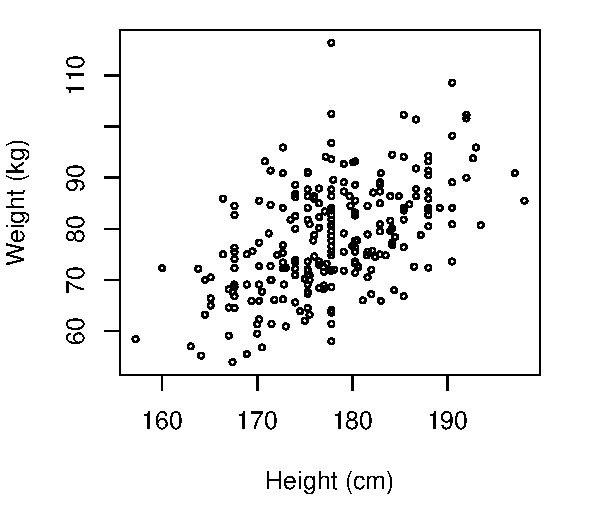
\includegraphics[scale=0.5]{figure/wgt_hgt_plot.pdf}
\end{figure}
\end{frame}

%-------------------------------------------
\begin{frame}{SLR Model}
Let $\{ (x_i, y_i) : i=1, \cdots, n \}$ be a collection of $n$ data points.  A \textbf{simple linear regression model} expressing the relationship between $Y_i$ and $x_i$ is given by:
$$ Y_i = \beta_0 + \beta_1 x_i + e_i $$
\begin{itemize}
\item $Y_i$ response variable (random)
\item $x_i$ explanatory variable (non-random)
\item $\beta_0$ intercept parameter (non-random)
\item $\beta_1$ slope parameter (non-random)
\item $e_i$ is the random error term; assume $e_i \sim N(0, \sigma^2)$\\ 
\end{itemize}
\vspace{10pt}

\footnotesize
\textbf{Remark:}  We capitalize $Y_i$ in the equation to emphasize that it is a random variable.  $Y_i$ is also sometimes called the \textbf{dependent} variable, and $x_i$ the \textbf{independent} or \textbf{predictor} variable.  Notation and terminology may vary depending on the textbook and context.
\end{frame}

%-------------------------------------------
\begin{frame}{Conditional Mean and Variance Functions}
\begin{itemize}
\item This expected value of $Y$ when $X$ takes a specific value $x$.
$$E(Y| X=x) = \beta_0 + \beta_1 x$$\\
For SLR, the conditional mean is modeled as a straight line. 
\vspace{5pt}

\item The variance of $Y$ when $X$ takes a specific value $x$.
$$Var(Y| X=x) = \sigma^2$$
An assumption for SLR is that the variance is the same for every value of $x$.  
\vspace{5pt}

\item The conditional distribution of $Y$ when $X$ takes takes a specific value $x$.
$$Y|X \sim N(\beta_0 + \beta_1 x, \sigma^2)$$
\end{itemize}
\end{frame}
% Show this from the normality assumption

\begin{frame}
\begin{figure}
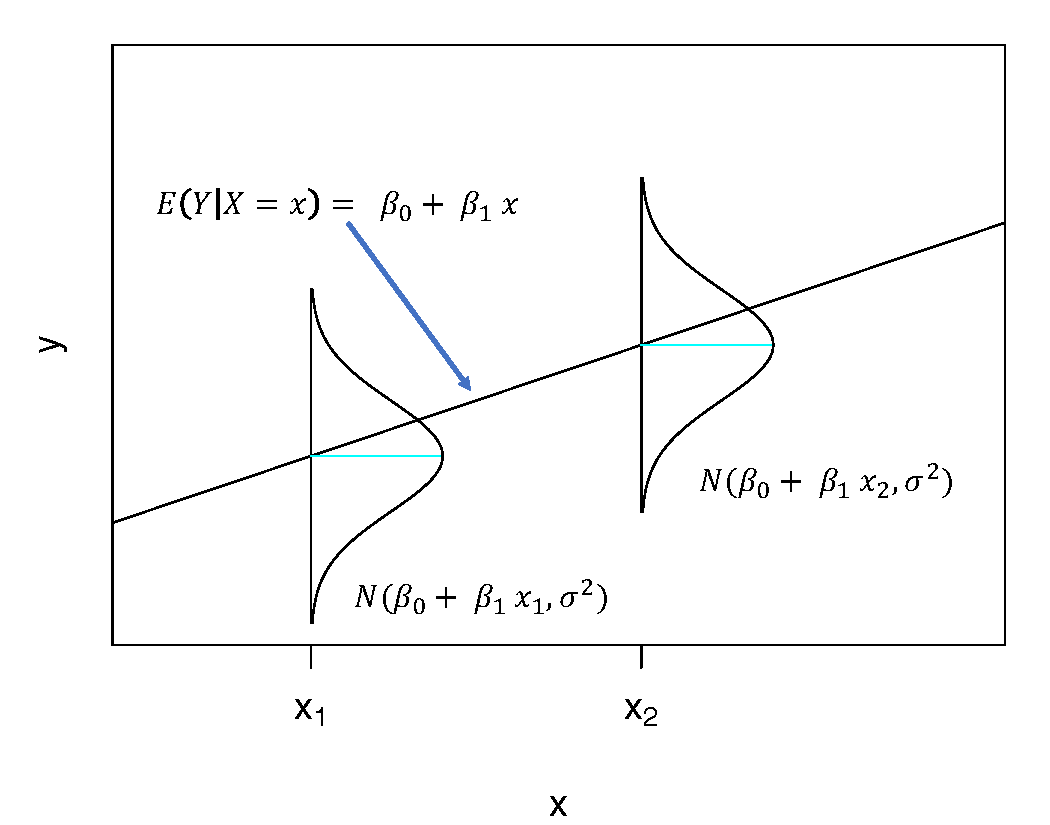
\includegraphics[scale=0.55]{figure/scatter_norm_annotated.pdf}
\end{figure}
\end{frame}

%-------------------------------------------
\begin{frame}{Fitted Values and Residuals}
The line that we estimate, or fit to the data in the scatterplot, is written~as
$$\hat{y} = \hat{\beta}_0 + \hat{\beta}_1 x$$\\
\vspace{10pt}

The fitted (or predicted) value for the $i^{th}$ observation $(x_i, y_i)$:
$$\hat{y}_i = \hat{\beta}_0 + \hat{\beta}_1 x_i$$\\
\vspace{10pt}

The \textbf{residual} for the $i^{th}$ observation is the difference between the observed value ($y_i$) and the predicted value ($\hat{y}_i$):\\
$$\hat{e}_i = y_i - \hat{y}_i = y_i - (\hat{\beta}_0 + \hat{\beta}_1 x_i)$$
\end{frame}

%-------------------------------------------
\begin{frame}
\begin{figure}
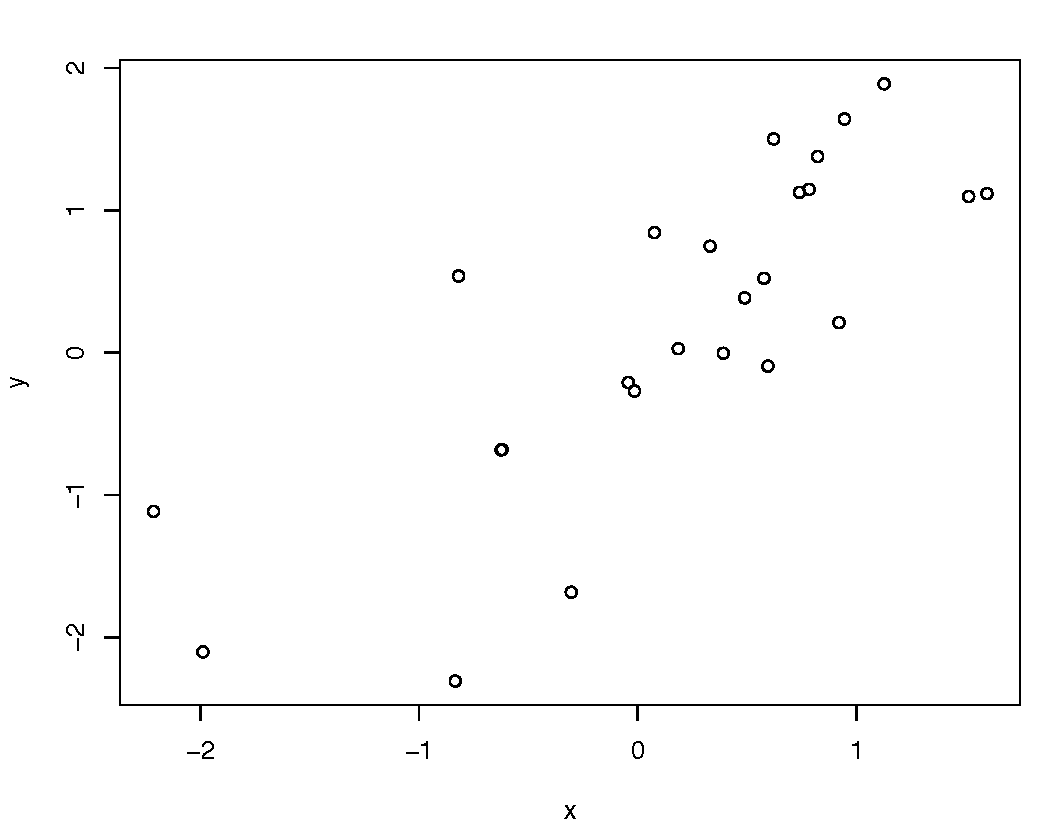
\includegraphics[scale=0.5]{figure/scatter1_2.pdf}
\end{figure}
\end{frame}

%-------------------------------------------
\begin{frame}
\begin{figure}
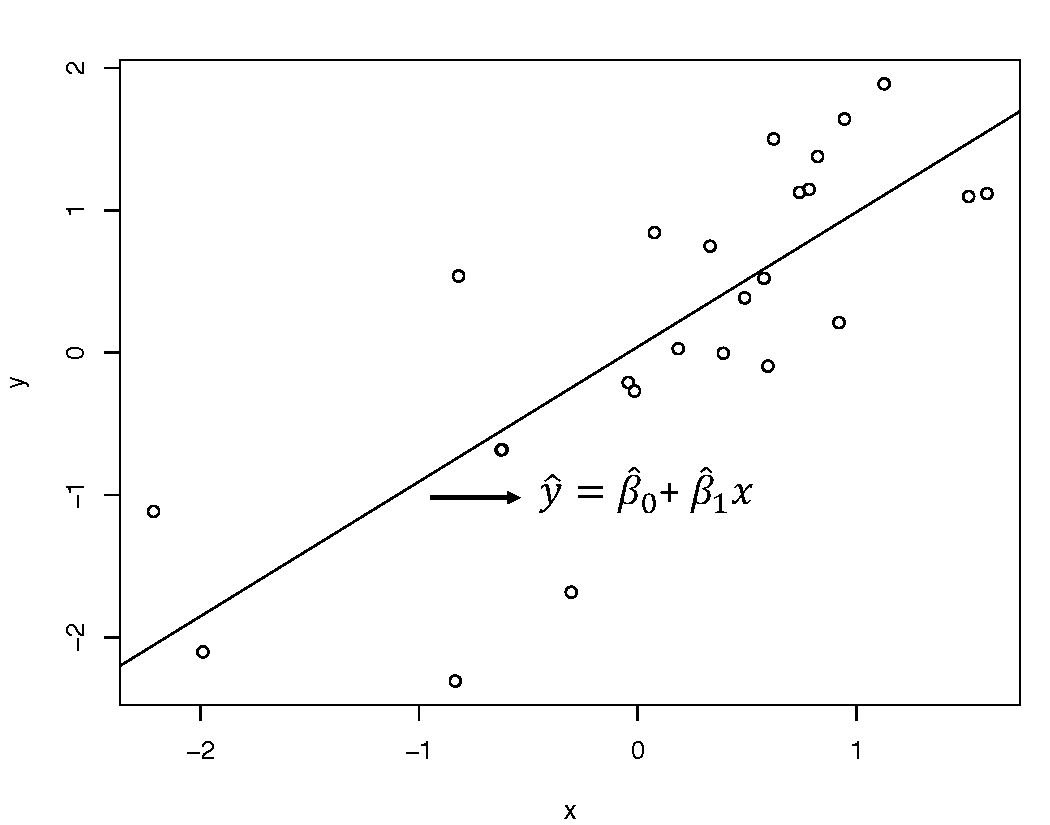
\includegraphics[scale=0.5]{figure/scatter2_2.pdf}
\end{figure}
\end{frame}

%-------------------------------------------
\begin{frame}
\begin{figure}
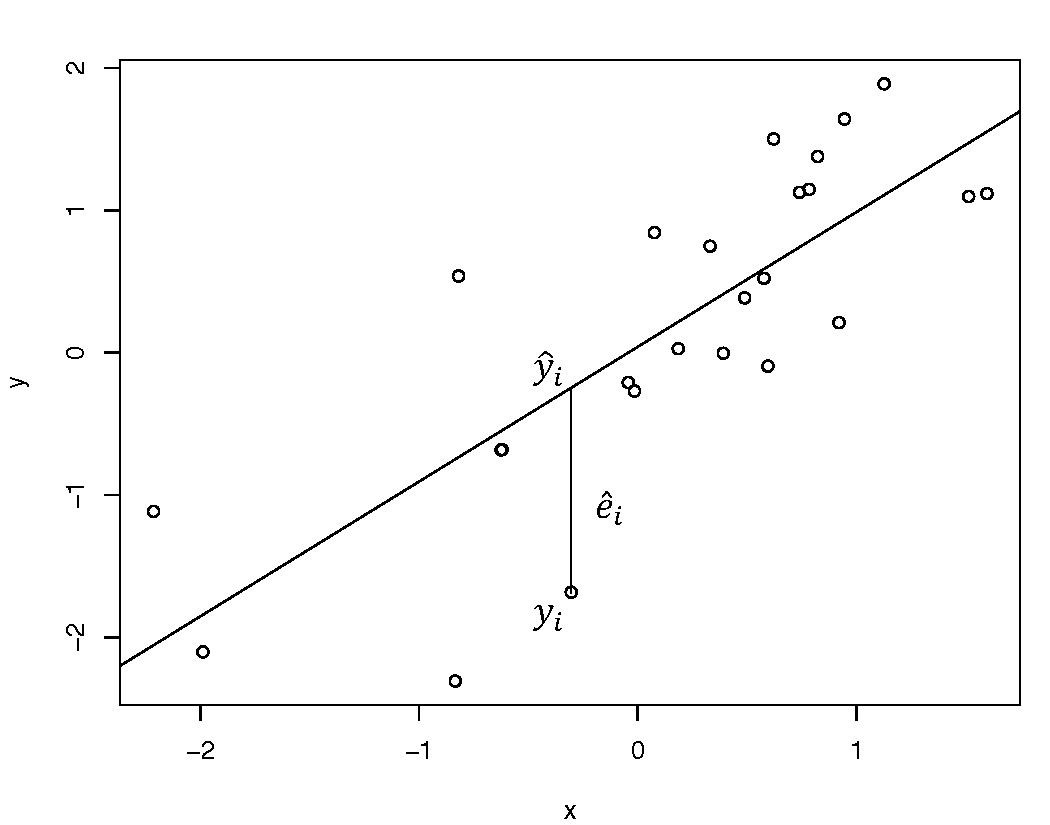
\includegraphics[scale=0.5]{figure/scatter3_2.pdf}
\end{figure}
\end{frame}

%-------------------------------------------
\begin{frame}
\begin{figure}
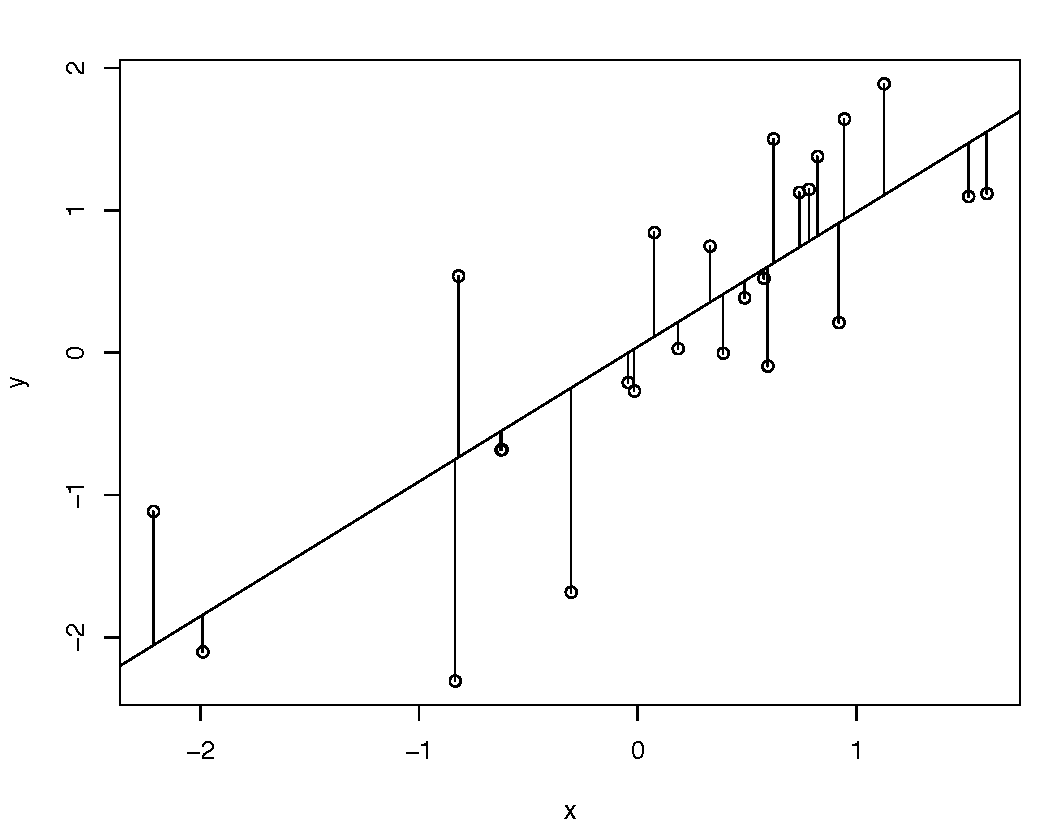
\includegraphics[scale=0.5]{figure/scatter4_2.pdf}
\end{figure}
\end{frame}

%-------------------------------------------
\begin{frame}{Sum of Squared Residuals}
\begin{itemize}
\item Intuitively, a line that fits the data well has small residuals.
\vspace{5pt}
\item The \textbf{least squares line} minimizes the \textbf{sum of squared residuals}:
$$RSS = \sum_{i=1}^n \hat{e}_i^2 = \sum_{i=1}^n (y_i - \hat{\beta}_0 - \hat{\beta}_1 x_i)^2$$
\vspace{5pt}
\item That is, out of all possible lines we could draw on the scatterplot, the least squares line is the ``best fit" since it has the smallest sum of squared residuals.
\end{itemize}
\end{frame}

%-------------------------------------------
\begin{frame}{Least Squares Estimation}
Formally, the estimates $\hat{\beta}_0$ and $\hat{\beta}_1$ of the intercept and slope are found by using calculus to minimize the sum of squared residuals:
\begin{align*}
RSS = \sum_{i=1}^n (y_i - \hat{\beta}_0 - \hat{\beta}_1 x_i)^2
\end{align*}

To minimize set the partial derivatives equal to zero:\\
\begin{align*}
\frac{\partial RSS}{\partial \hat{\beta}_0} &= -2 \sum_{i=1}^n (y_i - \hat{\beta}_0 - \hat{\beta}_1 x_i) = 0\\
\frac{\partial RSS}{\partial \hat{\beta}_1} &= -2 \sum_{i=1}^n x_i (y_i - \hat{\beta}_0 - \hat{\beta}_1 x_i) = 0
\end{align*}
\end{frame}

%-------------------------------------------
\begin{frame}{Least Squares Estimation}
Solving these two equations gives the \textbf{least squares estimates} of the intercept and slope:
\begin{align*}
\hat{\beta}_0 &= \bar{y} - \hat{\beta}_1 \bar{x}\\
\hat{\beta}_1 &= \frac{\sum_{i=1}^n x_iy_i - n\bar{x}\bar{y}}{\sum_{i=1}^n x_i^2 - n \bar{x}^2} = \frac{\sum_{i=1}^n (x_i - \bar{x})(y_i - \bar{y})}{\sum_{i=1}^n (x_i - \bar{x})^2} = \frac{SXY}{SXX} \end{align*}
Note that the equation for the intercept guarantees the least squares line passes through $(\bar{x}, \bar{y})$.
\end{frame}
% Solve equations on board
% Recall that the derivative of sum is sum of derivates

%------------------------------------------------------
\begin{frame}{Interpretation}
\begin{itemize}
\item \textbf{Slope}: an increase in the explanatory variable ($x$) by one unit is associated with a change of $\hat{\beta}_1$ in the predicted response ($\hat{y}$). 
\vspace{10pt}
\item \textbf{Intercept}: the prediction for the response variable ($\hat{y}$) when the value for the explanatory variable is zero ($x=0$).  It may not make sense to try to interpret the intercept depending on the application.    
\end{itemize}
\end{frame}

%-------------------------------------------
\begin{frame}{Estimating $\sigma^2$}
Estimate of $Var(e_i) = \sigma^2$:
\begin{align*}
\hat{\sigma}^2 = \frac{\text{RSS}}{n-2} = \frac{1}{n-2} \sum_{i=1}^n \hat{e}_i^2 = \frac{1}{n-2} \sum_{i=1}^n (y_i - \hat{y}_i)^2
\end{align*}
Remarks:
\begin{itemize}
\item $\sum_{i=1}^n \hat{e}_i = 0$ 
\item $\hat{\sigma} = \sqrt{RSS / (n-2)}$ called the \textbf{residual standard error}
\item The divisor is $n-2$ since two parameters $\beta_0$ and $\beta_1$ were estimated
\item It can be shown that $\hat{\sigma}^2$ is an unbiased estimate of $\sigma^2$, i.e, $E(\hat{\sigma}^2) = \sigma^2$
\end{itemize}
\end{frame}
% sketch proof (Weisberg, pg.27)

%-------------------------------------------
\begin{frame}[fragile]{Example}
\small
\begin{verbatim}
> lm1 <- lm(wgt ~ hgt, data=bdims_males)
> summary(lm1)

Coefficients:
             Estimate Std. Error t value Pr(>|t|)    
(Intercept) -60.95336   14.05436  -4.337 2.11e-05 ***
hgt           0.78257    0.07901   9.905  < 2e-16 ***
---
Signif. codes:  0 ‘***’ 0.001 ‘**’ 0.01 ‘*’ 0.05 ‘.’ 0.1 ‘ ’ 1

Residual standard error: 8.902 on 245 degrees of freedom
Multiple R-squared:  0.2859,	Adjusted R-squared:  0.283 
F-statistic: 98.11 on 1 and 245 DF,  p-value: < 2.2e-16
\end{verbatim}
\end{frame}

%-------------------------------------------
\begin{frame}[fragile]{Example}
A scatterplot of weight ($Y$) versus height ($X$) for 247 physically active men with least squares line superimposed.
\small
\begin{verbatim}
> plot(wgt ~ hgt, data=bdims_males, 
    xlab = 'Height (cm)' , ylab = 'Weight (kg)', cex=0.5)
> abline(lm1)
\end{verbatim}
\begin{figure}[htbp]
\centering
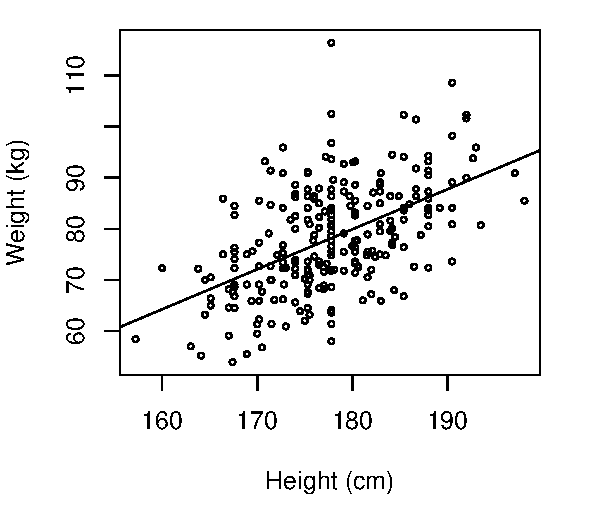
\includegraphics[scale=0.5]{figure/wgt_hgt_plot2.pdf}
\end{figure}
\end{frame}

%-------------------------------------------
\begin{frame}{Example}
\begin{itemize}
\item Equation of the least square regression line:\\
$\hat{y} = \hat{\beta}_0 + \hat{\beta}_1 x = -60.95 + 0.78 x$\\ 
or we can write $\widehat{\texttt{weight}} = -60.95 + 0.78 \texttt{height}$
\vspace{5pt}
\item Interpreting the slope: For men, an increase in height by 1 cm is associated with an increase in weight by 0.78 kg.
\vspace{5pt}
\item Interpreting the intercept:  The predicted weight for a man that is 0 cm tall is -60.95 kg.  Note that it does not makes sense to interpret the intercept in this context.  The prediction is an extrapolation (heights for men in this data set range between 157.2 to 198.1 cm).
\end{itemize}
\end{frame}

%-------------------------------------------
% \begin{frame}{Example - Your Turn}
% What is the predicted weight for a man that is 185 cm tall?\\
% \vspace{15pt}
% A man is this data set is 193.5 cm tall and weighs 80.7 km.  Calculate the residual for this individual? 
% \end{frame}


%-------------------------------------------
\begin{frame}[fragile]{Example}
We can calculate the residual standard error manually in R. This value is also given in the regression summary. 
\small
\begin{verbatim}
> n <- nrow(bdims_males)
> sqrt(sum(resid(lm1)^2) / (n-2))
[1] 8.901667
\end{verbatim}
\vspace{10pt}

\normalsize
Note that the empirical sum of the residuals is approximately 0:
\small
\begin{verbatim}
> sum(resid(lm1))
[1] -1.273981e-13
\end{verbatim}
\end{frame}
% make to a prediction and residual calculation on the board


%-------------------------------------------
\begin{frame}{Partitioning Variability}
Graphical description that $y_i - \bar{y} = (y_i - \hat{y}_i) + (\hat{y}_i - \bar{y})$

\begin{figure}
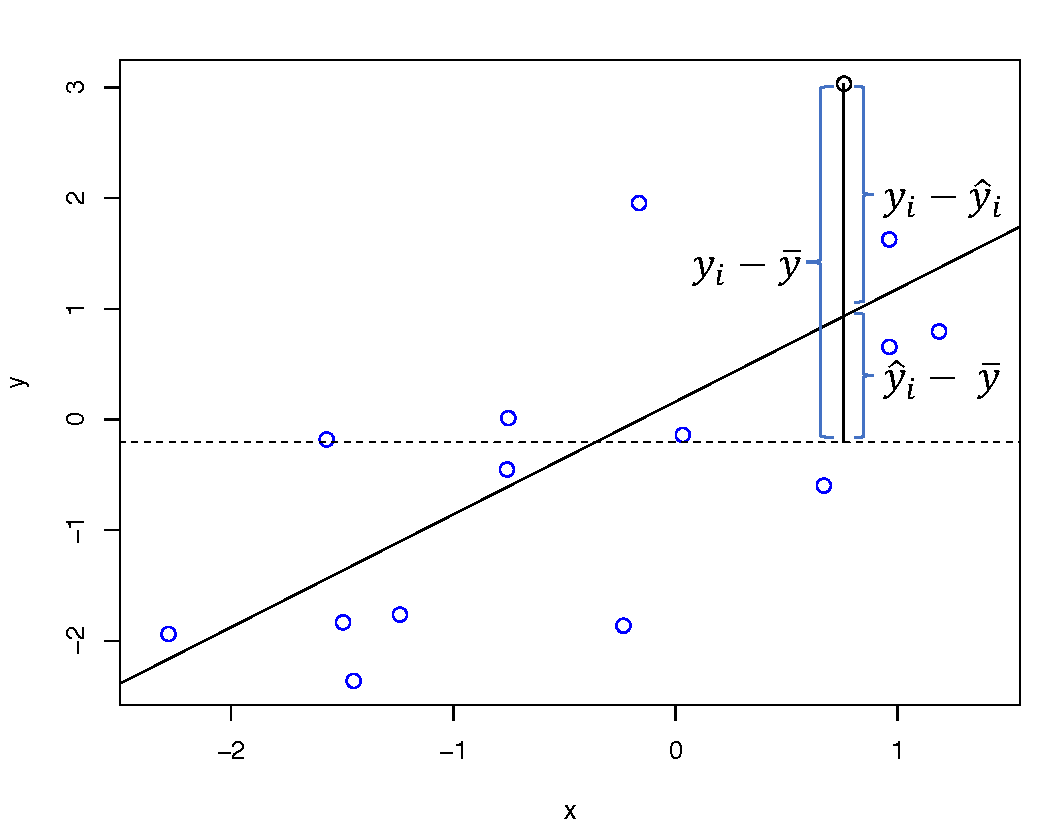
\includegraphics[scale=0.4]{figure/partition_variance2.pdf}
\end{figure}
\end{frame}

\begin{frame}{Partitioning Variability}
Remarkably, it can be shown that
\begin{align*}
\sum_{i=1}^n (y_i - \bar{y})^2 &= \sum_{i=1}^n (\hat{y}_i - \bar{y})^2 + \sum_{i=1}^n (y_i - \hat{y}_i)^2\\
\text{SST} &= \text{SSreg} + \text{RSS}
\end{align*}
\begin{itemize}
\item SST is the total sum of squares (total variability in the response variable)
\item SSreg is the regression sum of squares (variability in the response explained by the model)
\item RSS is the residual sum of squares (unexplained variability)
\end{itemize}
\end{frame}

%-------------------------------------------
\begin{frame}{Coefficient of Determination}
The \textbf{coefficient of determination} ($R^2$) is a measure of how well the linear regression model fits the data.
\begin{align*}
R^2 = \frac{\text{SSReg}}{\text{SST}} = 1 - \frac{\text{RSS}}{\text{SST}}
\end{align*}
\vspace{10pt}
\begin{itemize}
\item $R^2$ can be interpreted as the proportion of variability in the response variable $Y$ that is explained by $X$ (i.e., the regression model).
\vspace{5pt}
\item $0 \leq R^2 \leq 1$; the closer $R^2$ is to 1, the better the linear regression model fits the data.
\vspace{5pt}
\item For the example, $R^2 = 0.286$ (see summary output), meaning that for men, 28.6\% of the variability in weight can be explained by height.
\end{itemize}
\end{frame}
% can show computation on board

%-------------------------------------------
\begin{frame}
Limiting cases:
\begin{itemize}
\item $R^2 = 1$ when all points fall on the regression line (RSS=0)
\item $R^2 = 0$ when $\hat{y}_i = \bar{y}$, which implies RSS=SST.
\end{itemize}
\centering
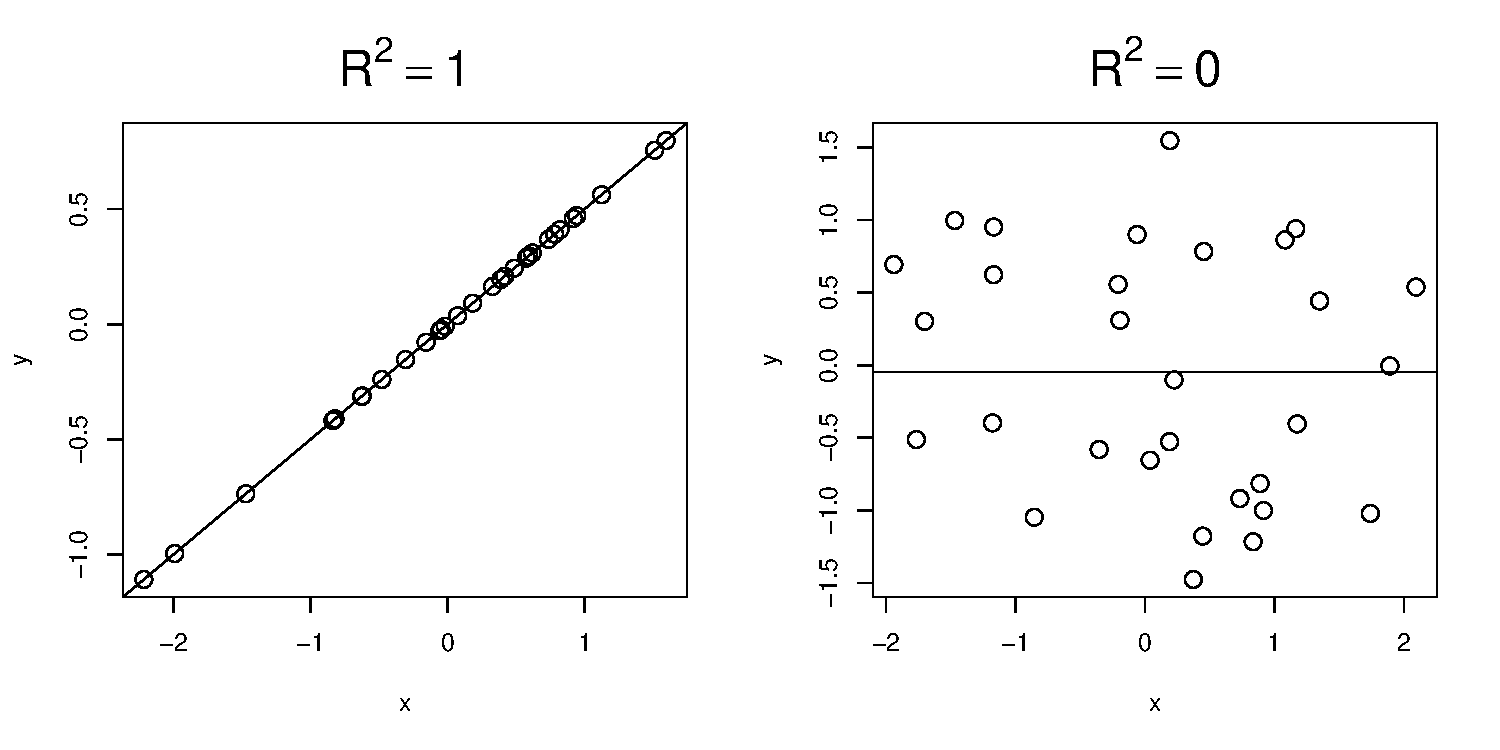
\includegraphics[scale=0.4]{figure/R2.pdf}
\end{frame}

%-------------------------------------------
\begin{frame}{Correlation Coefficient (review)}
The \textbf{correlation coefficient}, denoted by $r$, is a number between -1 and 1 that describes the strength of the linear association between two variables.

\begin{align*}
r = \frac{\sum_{i=1}^n (x_i - \bar{x}) (y_i - \bar{y})}{\sqrt{\sum_{i=1}^n (x_i - \bar{x})^2} \sqrt{\sum_{i=1}^n (y_i - \bar{y})^2}} = \frac{1}{n-1} \sum_{i=1}^n \left(\frac{x_i - \bar{x}}{s_x} \right) \left( \frac{y_i - \bar{y}}{s_y} \right)
\end{align*}
\begin{itemize}
\item $\bar{x}$ and $\bar{y}$ are the sample means
\item $s_x$ and $s_y$ are the sample standard deviations
\end{itemize}
\end{frame}

%-------------------------------------------
\begin{frame}{Correlation Coefficent}
\begin{figure}
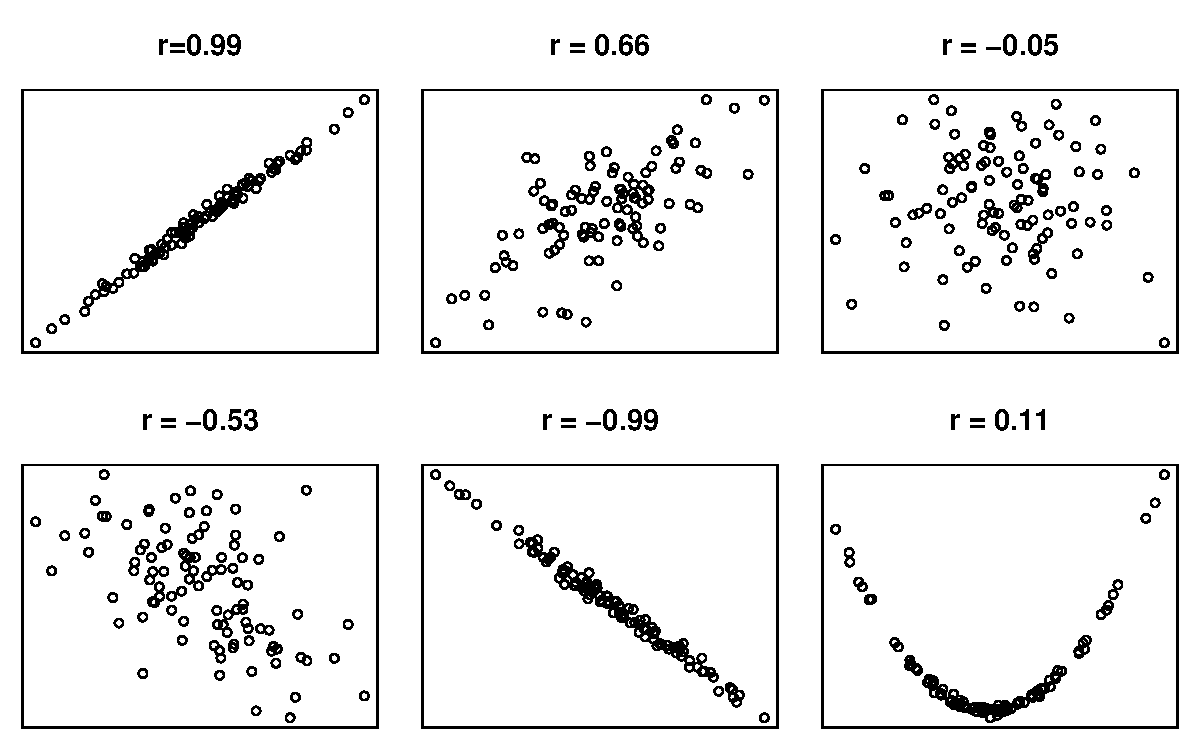
\includegraphics[scale=0.5]{figure/correlations.pdf}
\end{figure}
\end{frame}

%-------------------------------------------
\begin{frame}{Correlation Coefficient}
\begin{itemize}
\item $r \approx 1$ when there is a strong positive linear association between the variables.
\vspace{5pt}
\item $r \approx -1$ when there is a strong negative linear association between the variables.
\vspace{5pt}
\item $r \approx 0$ when there is no association between the variables (i.e., independent).
\vspace{5pt}
\item The correlation coefficient is only useful for evaluating the linear association between two variables.  It is not a useful measure for nonlinear relationships.
\end{itemize}
\end{frame}

%-------------------------------------------
\begin{frame}[fragile]{Correlation Coefficent}
\begin{itemize}
\item $R^2$ can also be computed as the correlation coefficient squared.
\begin{verbatim}
> cor(bdims_males$wgt, bdims_males$hgt)^2
[1] 0.2859487
\end{verbatim}
\vspace{10pt}
\item The least squares estimate of the slope can be written in terms of the the correlation coefficient:
$$\hat{\beta}_1 = r \frac{s_y}{s_x}$$
\end{itemize}
\end{frame}

\end{document}